\documentclass{oblivoir}
%%%Default packages
\usepackage{amsmath,amssymb,amsthm,kotex,tabu,graphicx,pifont}
\usepackage{../kswrapfig}

\usepackage{gensymb} %\degree

%%%More packages
%\usepackage{caption,subcaption}
%\usepackage[perpage]{footmisc}
%
\usepackage[skipabove=10pt,innertopmargin=10pt,nobreak=true]{mdframed}

\usepackage[inline]{enumitem}
\setlist[enumerate,1]{label=(\arabic*)}
\setlist[enumerate,2]{label=(\alph*)}

\usepackage{multicol}
\setlength{\columnsep}{30pt}
\setlength{\columnseprule}{1pt}
%
%\usepackage{forest}
%\usetikzlibrary{shapes.geometric,arrows.meta,calc}
%
%%%defi theo exam prob rema proo
%이 환경들 아래에 문단을 쓸 경우 살짝 들여쓰기가 되므로 \hspace{-.7em}가 필요할 수 있다.

\newcounter{num}
\newcommand{\defi}[1]
{\noindent\refstepcounter{num}\textbf{정의 \arabic{num})} #1\par\noindent}
\newcommand{\theo}[1]
{\noindent\refstepcounter{num}\textbf{정리 \arabic{num})} #1\par\noindent}
\newcommand{\revi}[1]
{\noindent\refstepcounter{num}\textbf{복습 \arabic{num})} #1\par\noindent}
\newcommand{\exam}[1]
{\bigskip\bigskip\noindent\refstepcounter{num}\textbf{예시 \arabic{num})} #1\par\noindent}
\newcommand{\prob}[1]
{\bigskip\bigskip\noindent\refstepcounter{num}\textbf{문제 \arabic{num})} #1\par\noindent}
\newcommand{\rema}[1]
{\bigskip\bigskip\noindent\refstepcounter{num}\textbf{참고 \arabic{num})} #1\par\noindent}
\newcommand{\proo}
{\bigskip\noindent\textsf{증명)}}

\newenvironment{talign}
 {\let\displaystyle\textstyle\align}
 {\endalign}
\newenvironment{talign*}
 {\let\displaystyle\textstyle\csname align*\endcsname}
 {\endalign}
%
%%%Commands

\newcommand{\procedure}[1]{\begin{mdframed}\vspace{#1\textheight}\end{mdframed}}

\newcommand\an[1]{\par\bigskip\noindent\textbf{문제 \ref{#1})}\par\noindent}

\newcommand\ann[2]{\par\bigskip\noindent\textbf{문제 \ref{#1})}\:\:#2\par\medskip\noindent}

\newcommand\ans[1]{\begin{flushright}\textbf{답 : }#1\end{flushright}}

\newcommand\anssec[1]{\bigskip\bigskip\noindent{\large\bfseries#1}}

\newcommand{\pb}[1]%\Phantom + fBox
{\fbox{\phantom{\ensuremath{#1}}}}

\newcommand\ba{\,|\,}

\newcommand\ovv[1]{\ensuremath{\overline{#1}}}
\newcommand\ov[2]{\ensuremath{\overline{#1#2}}}
%
%%%% Settings
%\let\oldsection\section
%
%\renewcommand\section{\clearpage\oldsection}
%
%\let\emph\textsf
%
%\renewcommand{\arraystretch}{1.5}
%
%%%% Footnotes
%\makeatletter
%\def\@fnsymbol#1{\ensuremath{\ifcase#1\or
%*\or **\or ***\or
%\star\or\star\star\or\star\star\star\or
%\dagger\or\dagger\dagger\or\dagger\dagger\dagger
%\else\@ctrerr\fi}}
%
%\renewcommand{\thefootnote}{\fnsymbol{footnote}}
%\makeatother
%
%\makeatletter
%\AtBeginEnvironment{mdframed}{%
%\def\@fnsymbol#1{\ensuremath{\ifcase#1\or
%*\or **\or ***\or
%\star\or\star\star\or\star\star\star\or
%\dagger\or\dagger\dagger\or\dagger\dagger\dagger
%\else\@ctrerr\fi}}%
%}   
%\renewcommand\thempfootnote{\fnsymbol{mpfootnote}}
%\makeatother
%
%%% 객관식 선지
\newcommand\one{\ding{172}}
\newcommand\two{\ding{173}}
\newcommand\three{\ding{174}}
\newcommand\four{\ding{175}}
\newcommand\five{\ding{176}}
\usepackage{tabto,pifont}
%\TabPositions{0.2\textwidth,0.4\textwidth,0.6\textwidth,0.8\textwidth}

\newcommand\taba[5]{\par\noindent
\one\:{#1}
\tabto{0.2\textwidth}\two\:\:{#2}
\tabto{0.4\textwidth}\three\:\:{#3}
\tabto{0.6\textwidth}\four\:\:{#4}
\tabto{0.8\textwidth}\five\:\:{#5}}

\newcommand\tabb[5]{\par\noindent
\one\:{#1}
\tabto{0.33\textwidth}\two\:\:{#2}
\tabto{0.67\textwidth}\three\:\:{#3}\medskip\par\noindent
\four\:\:{#4}
\tabto{0.33\textwidth}\five\:\:{#5}}

\newcommand\tabc[5]{\par\noindent
\one\:{#1}
\tabto{0.5\textwidth}\two\:\:{#2}\medskip\par\noindent
\three\:\:{#3}
\tabto{0.5\textwidth}\four\:\:{#4}\medskip\par\noindent
\five\:\:{#5}}

\newcommand\tabd[5]{\par\noindent
\one\:{#1}\medskip\par\noindent
\two\:\:{#2}\medskip\par\noindent
\three\:\:{#3}\medskip\par\noindent
\four\:\:{#4}\medskip\par\noindent
\five\:\:{#5}}
%
%%%% fonts
%
%\usepackage{fontspec, xunicode, xltxtra}
%\setmainfont[]{은 바탕}
%\setsansfont[]{은 돋움}
%\setmonofont[]{은 바탕}
%\XeTeXlinebreaklocale "ko"
%%%%
\begin{document}

\title{수학(하) : 04 내분점과 외분점}
\author{}
\date{\today}
\maketitle
\tableofcontents
\newpage

%%%
\section{내분점과 외분점(1차원)}

%
\begin{mdframed}
\defi{내분점과 외분점}
선분 \(\ov AB\)위의 점 \(P\)가
\[\ov AP:\ov PB=m:n\]
를 만족시키면, 점 \(P\)를 점 \(A\)와 점 \(B\)의 \(m:n\) \emph{내분점}이라고 한다.
\par\bigskip\noindent
선분 \(\ov AB\)의 연장선 위의 점 \(Q\)가
\[\ov AQ:\ov QB=m:n\]
를 만족시키면, 점 \(Q\)를 점 \(A\)와 점 \(B\)의 \(m:n\) \emph{외분점}이라고 한다.
\end{mdframed}

%
\exam{}\label{int01}
수직선 위의 두 점 \(A(1)\), \(B(7)\)에 대해\\
(1) \(A\)와 \(B\)의 \(2:1\) 내분점은 \(P(5)\)이다.\par
\begin{center}
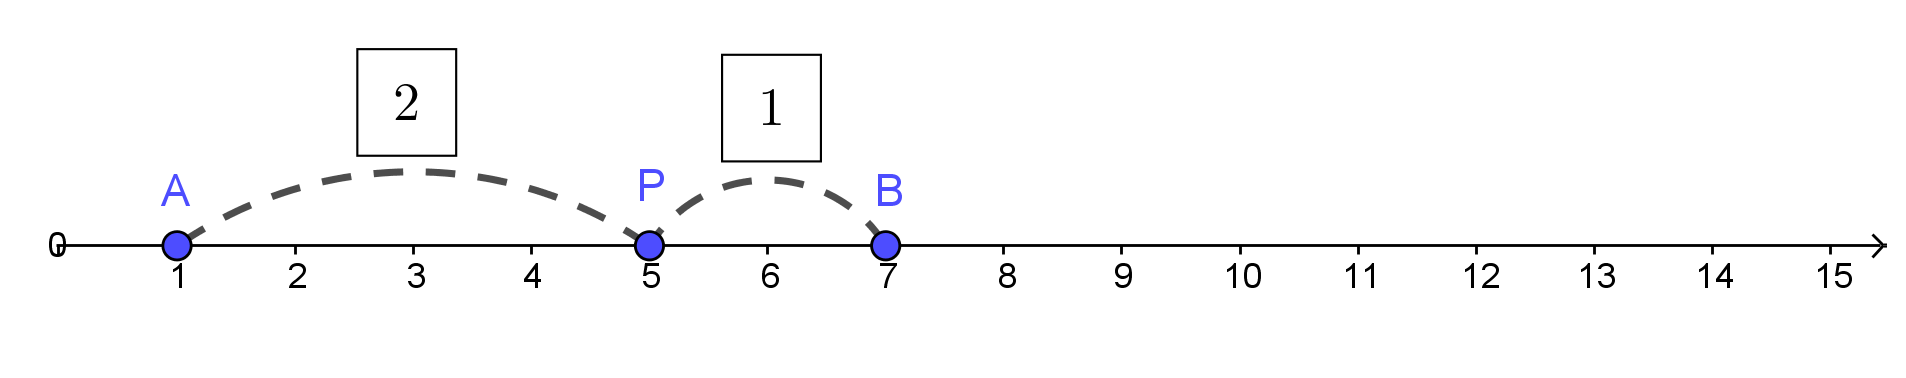
\includegraphics[width=0.7\textwidth]{int_01}
\end{center}
(2) \(A\)와 \(B\)의 \(2:1\) 외분점은 \(Q(13)\)이다.
\begin{center}
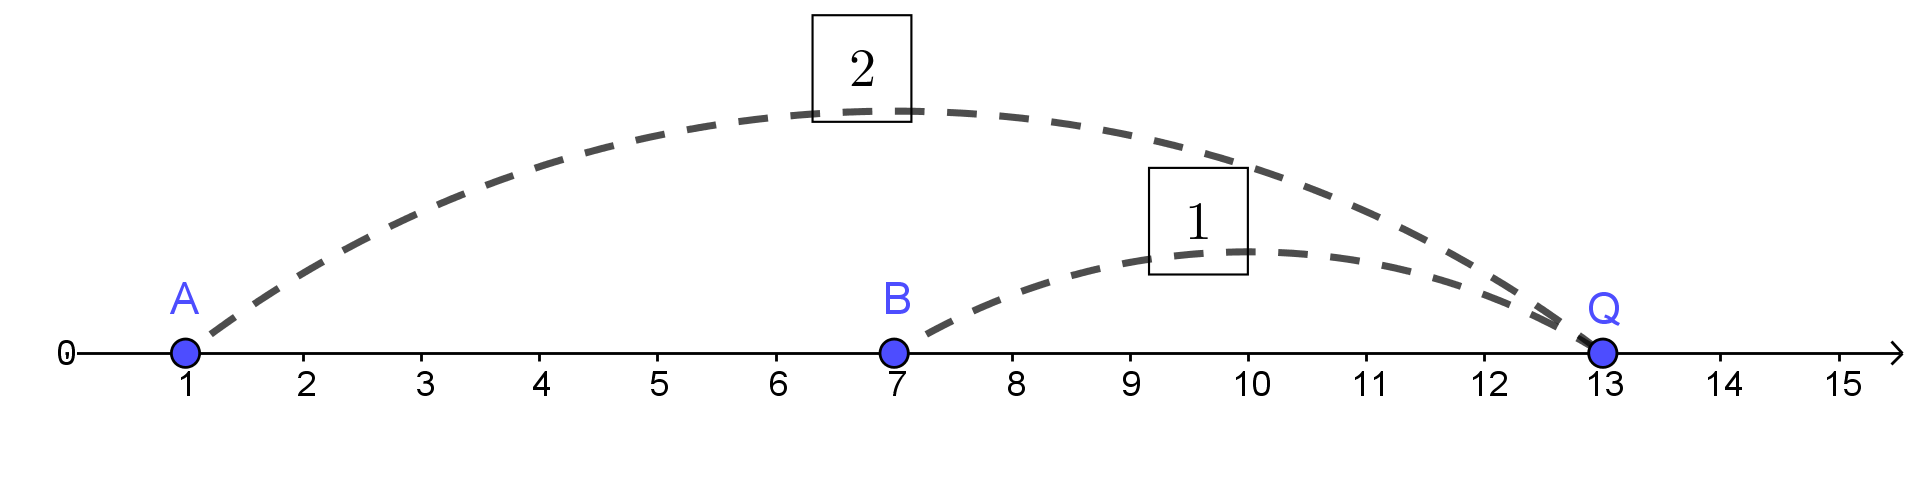
\includegraphics[width=0.7\textwidth]{int_02}
\end{center}

%
\prob{}\label{int03}
수직선 위의 두 점 \(A(2)\), \(B(10)\)에 대해\\
(1) \(A\)와 \(B\)의 \(3:1\) 내분점 \(P\)\\
(2) \(A\)와 \(B\)의  \(3:1\) 외분점 \(Q\)\\
(3) \(A\)와 \(B\)의 \(1:2\) 외분점 \(R\)\\
의 좌표를 각각 구하여라.

\clearpage
%
\exam{}\label{int04}
예시 \ref{int01})를 다음과 같이 풀어보자.
\(P\)의 좌표를 \(p\)라고 두면 \(P\)는 \(A\)와 \(B\) 사이에 있으므로 \(1<p<7\)이다.
\begin{center}
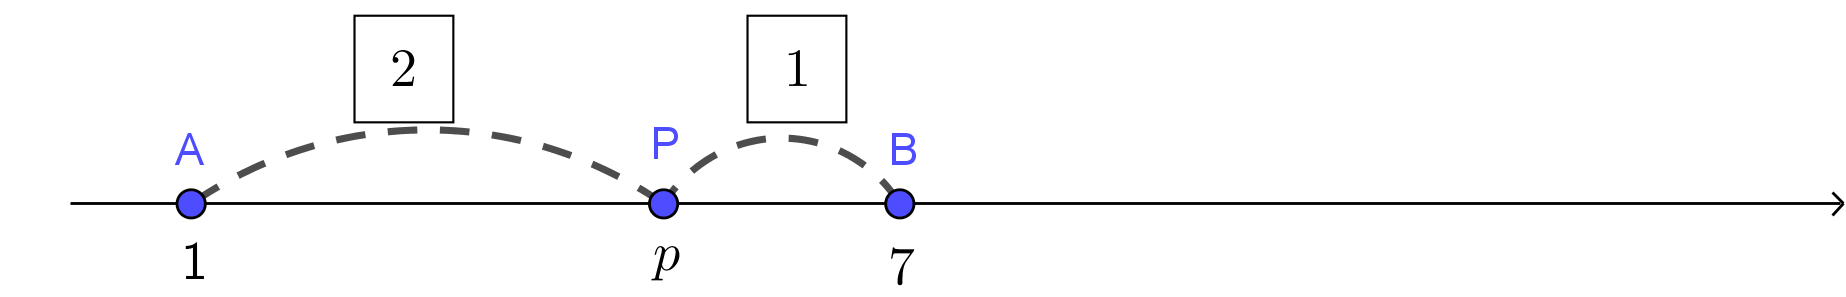
\includegraphics[width=0.7\textwidth]{int_04}
\end{center}
\(\ov AP=p-1\), \(\ov PB=7-p\)로부터
\begin{gather*}
p-1:7-p=2:1\\
2(7-p)=p-1\\
14-2p=p-1\\
3p=15\\
p=5
\end{gather*}
따라서 \(P\)의 좌표는 \(5\)이다.

\medskip
한편, \(Q\)의 좌표를 \(q\)라고 두면 \(Q\)는 \(B\)의 오른편에 있으므로 \(1<7<q\)이다.
\begin{center}
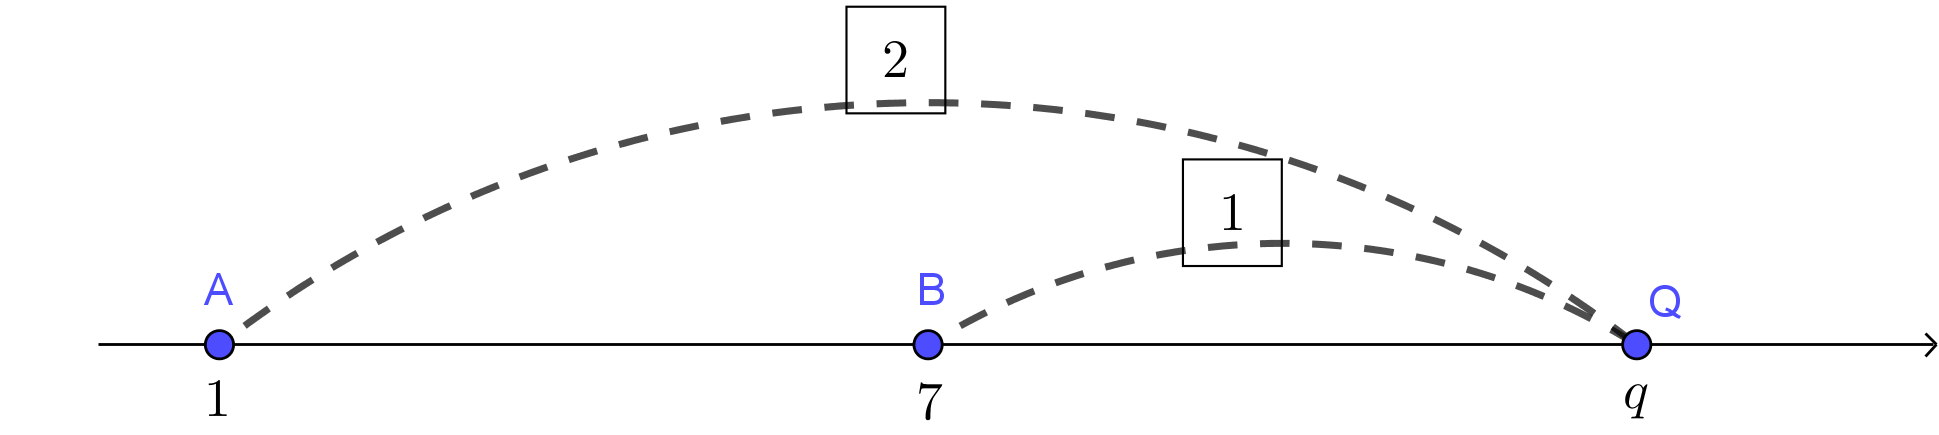
\includegraphics[width=0.7\textwidth]{int_05}
\end{center}
\(\ov AQ=q-1\), \(\ov QB=q-7\)로부터
\begin{gather*}
q-1:q-7=2:1\\
2(q-7)=q-1\\
2q-14=q-1\\
q=13
\end{gather*}
따라서 \(Q\)의 좌표는 \(13\)이다.

%
\prob{}\label{int06}
문제 \ref{int03})을 예시 \ref{int04})의 방법을 사용하여 풀어라.
\clearpage

\bigskip
%
\begin{mdframed}
\theo{내분점과 외분점의 좌표(1차원)}\label{int07}
두 점 \(A(a)\), \(B(b)\)에 대하여
\(A\)와 \(B\)의 \(m:n\) 내분점 \(P(p)\), 외분점 \(Q(q)\)의 좌표는 각각
\[p=\frac{mb+na}{m+n}\]
\[q=\frac{mb-na}{m-n}\]
이다.
\end{mdframed}
\[
p=\frac n{m+n}a+\frac m{m+n}b,
\qquad\qquad
q=-\frac n{m-n}a+\frac m{m-n}b
\]
로 쓸 수도 있다.

\proo
\bigskip\noindent\fbox{내분점 \(P\)}\par
\(P\)는 \(A\)와 \(B\) 사이에 있으므로 \(a<p<b\)이다.
\(\ov AP=p-a\), \(\ov PB=b-p\)로부터
\begin{center}
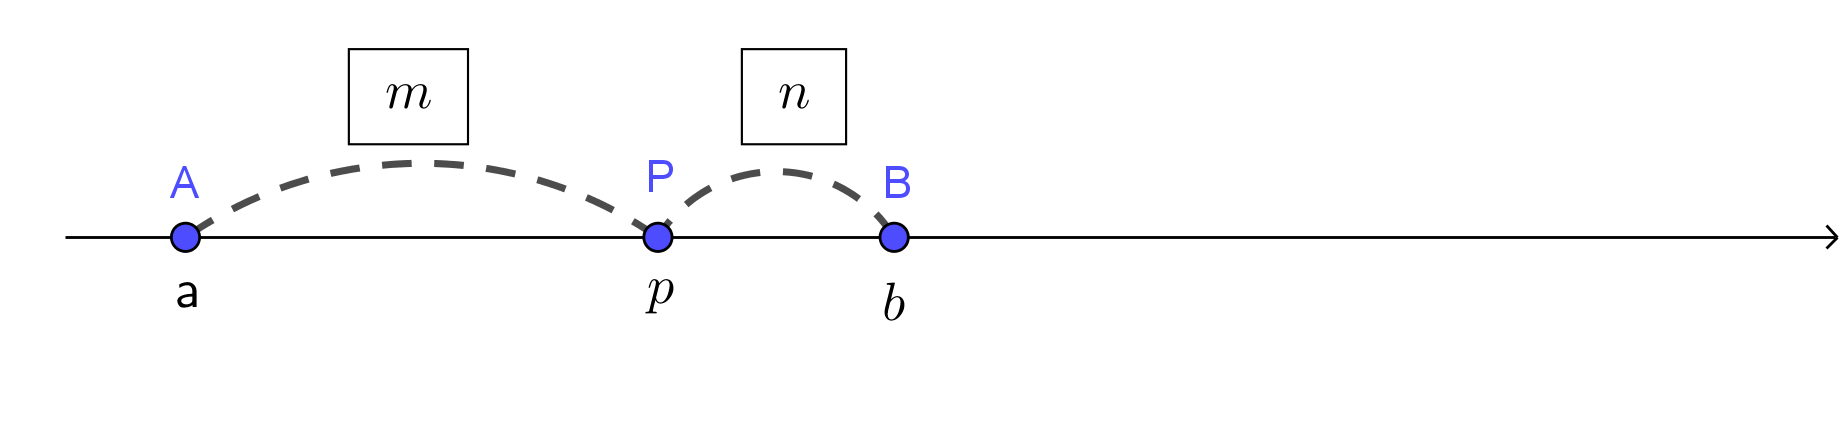
\includegraphics[width=0.7\textwidth]{int_07}
\end{center}
따라서
\begin{gather*}
p-a:b-p=m:n\\
m(b-p)=n(p-a)\\
mb-mp=np-na\\
mb+na=(m+n)p\\
p=\frac{mb+na}{m+n}
\end{gather*}
\qed

\clearpage
\bigskip\noindent\fbox{외분점 \(Q\)}\par
i) \(m>n\)일 때,\\
\(Q\)는 \(B\)의 오른편에 있으므로 \(a<b<q\)이다.
\begin{center}
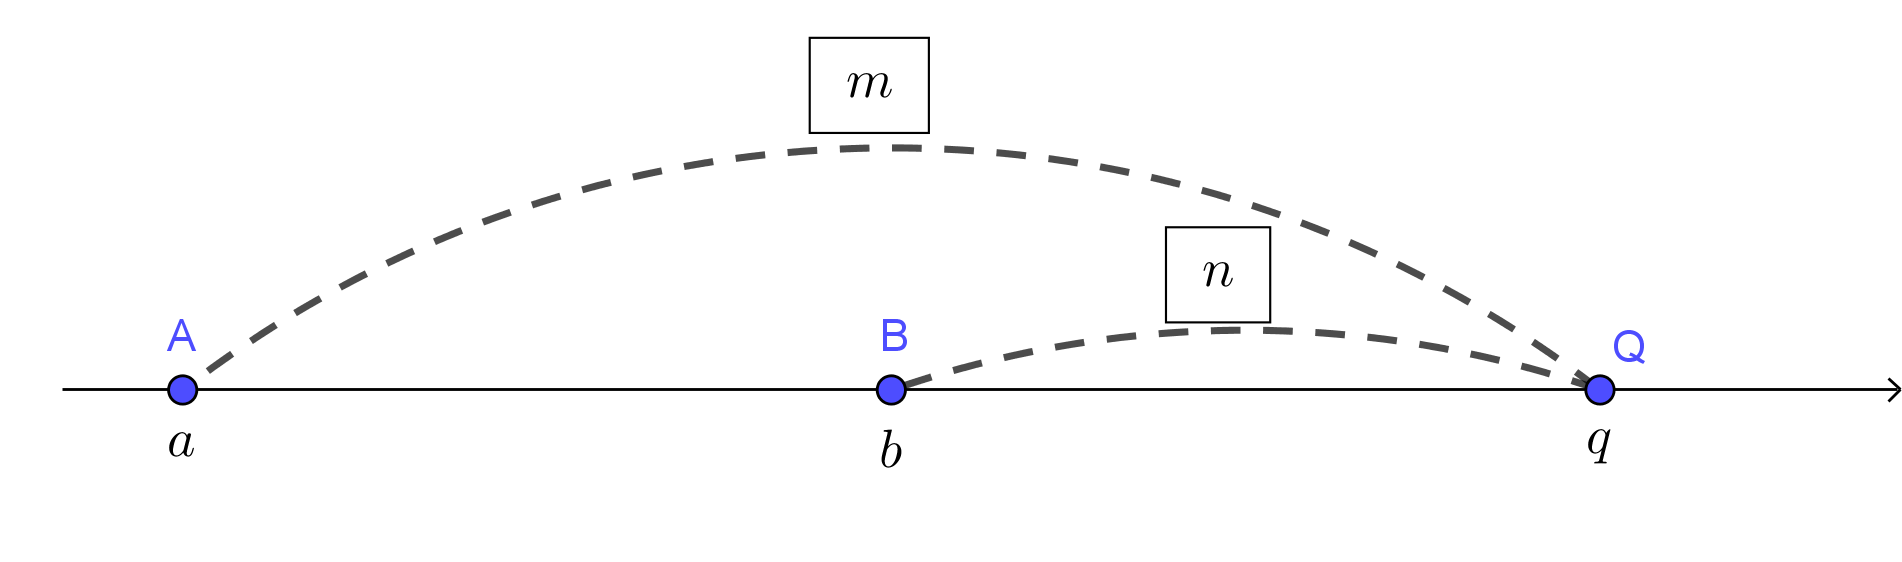
\includegraphics[width=0.7\textwidth]{int_08}
\end{center}
\(\ov AQ=q-a\), \(\ov QB=q-b\)로부터
\begin{gather*}
q-a:q-b=m:n\\
m(q-b)=n(q-a)\\
mq-mb=nq-na\\
(m-n)q=mb-na\\
q=\frac{mb-na}{m-n}
\end{gather*}

ii) \(m<n\)일 때,\\
\(Q\)는 \(B\)의 왼편에 있으므로 \(q<a<b\)이다.
\begin{center}
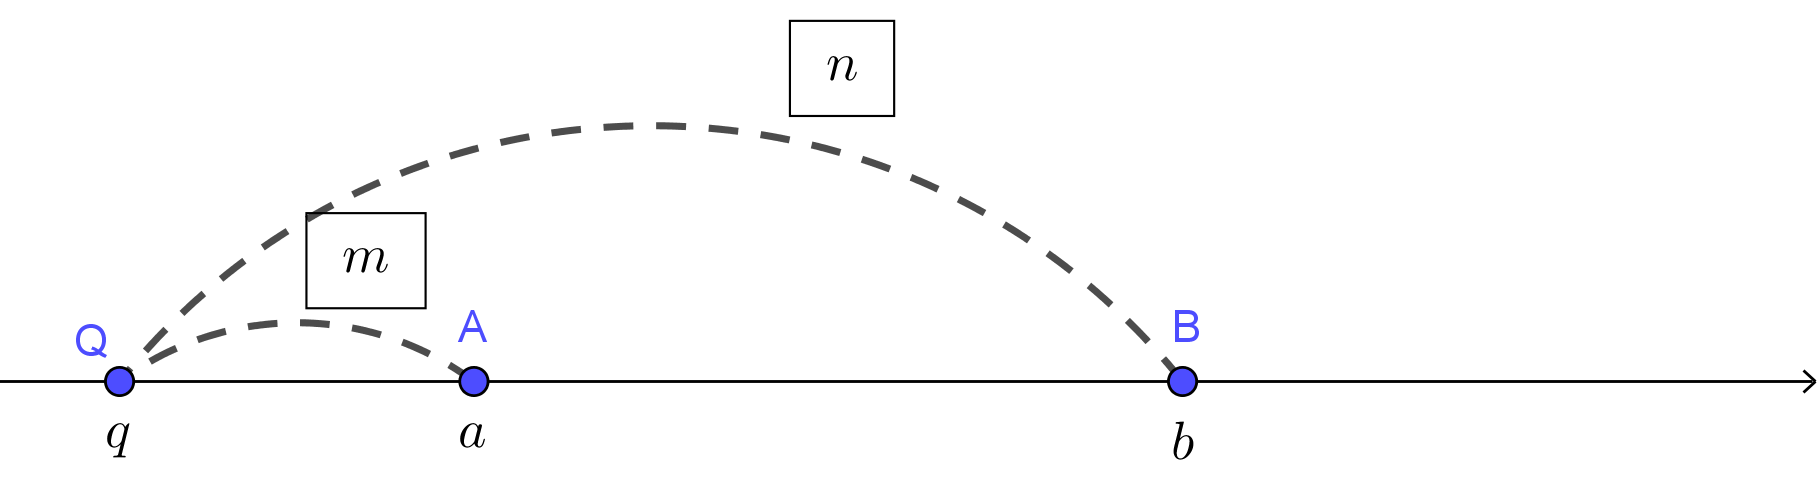
\includegraphics[width=0.7\textwidth]{int_09}
\end{center}
\(\ov AQ=a-q\), \(\ov QB=b-q\)로부터
\begin{gather*}
a-q:b-q=m:n\\
m(b-q)=n(a-q)\\
mb-mq=na-nq\\
mb-na=(m-n)q\\
q=\frac{mb-na}{m-n}
\end{gather*}
\qed

%
\exam{}
예시 \ref{int01})를
 정리 \ref{int07})의 공식을 사용해서 풀어보면
\begin{gather*}
p=\frac{2\times7+1\times1}{2+1}=\frac{15}3=5\\
q=\frac{2\times7-1\times1}{2-1}=\frac{13}1=13
\end{gather*}
이다.

%
\prob{}\label{int10}
문제 \ref{int03})을 정리 \ref{int07})의 공식을 사용하여 풀어라.

%
\prob{}\label{int11}
\(A(-1)\), \(B(5)\), \(C(8)\)에 대하여 다음 문장을 완성하여라.
\begin{enumerate}
\item
\(A\)는 \(B\)와 \(C\)의 \(\pb4:\pb4\) 외분점이다.
\item
\(B\)는 \(A\)와 \(C\)의 \(\pb4:\pb4\) 내분점이다.
\item
\(C\)는 \(A\)와 \(B\)의 \(\pb4:\pb4\) 외분점이다.
\end{enumerate}
\begin{center}
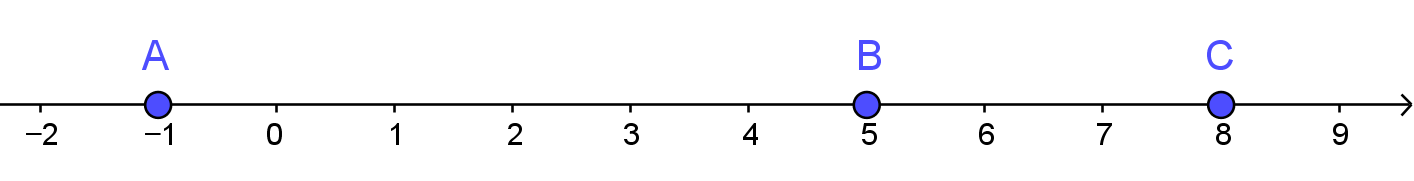
\includegraphics[width=0.6\textwidth]{int_11}
\end{center}

%
\prob{}\label{int12}
\(P(9)\)는 \(A(3)\)와 \(B(b)\)의 \(2:3\) 내분점이다.
이때 \(b\)의 값을 구하시오.
\procedure{0.1}

%
\prob{}\label{int13}
\(Q(11)\)는 \(A(a)\)와 \(B(5)\)의 \(4:3\) 외분점이다.
이때 \(a\)의 값을 구하시오.
\procedure{0.1}

%
\prob{}\label{int14}
선분 \(\ov AB\) 위의 두 점 \(P\), \(Q\)에 대해 \(P\)는 \(A\)와 \(B\)의 중점이고 \(Q\)는 \(A\)와 \(B\)의 2:1 내분점일 때, \(\ov AP:\ov PQ:\ov QB\)를 가장 간단한 자연수의 비로 나타내어라.
\begin{center}
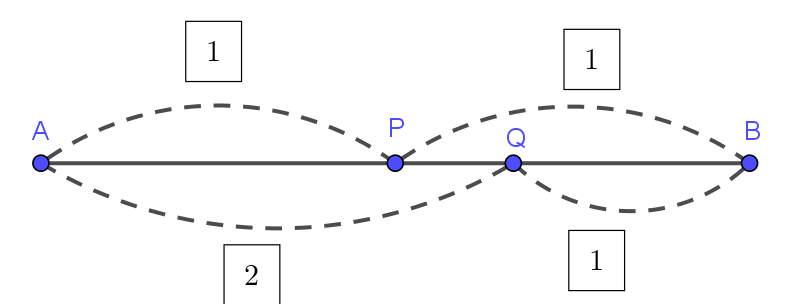
\includegraphics[width=0.6\textwidth]{int_14}
\end{center}
\procedure{0.1}

%
\prob{}\label{int15}
직선 \(\ov AB\) 위의 두 점 \(P\), \(Q\)에 대해 \(P\)는 \(A\)와 \(B\)의 \(3:2\) 내분점이고 \(Q\)는 \(A\)와 \(B\)의 \(3:2\) 외분점일 때, \(\ov AP:\ov PB:\ov BQ\)를 가장 간단한 자연수의 비로 나타내어라.
\begin{center}
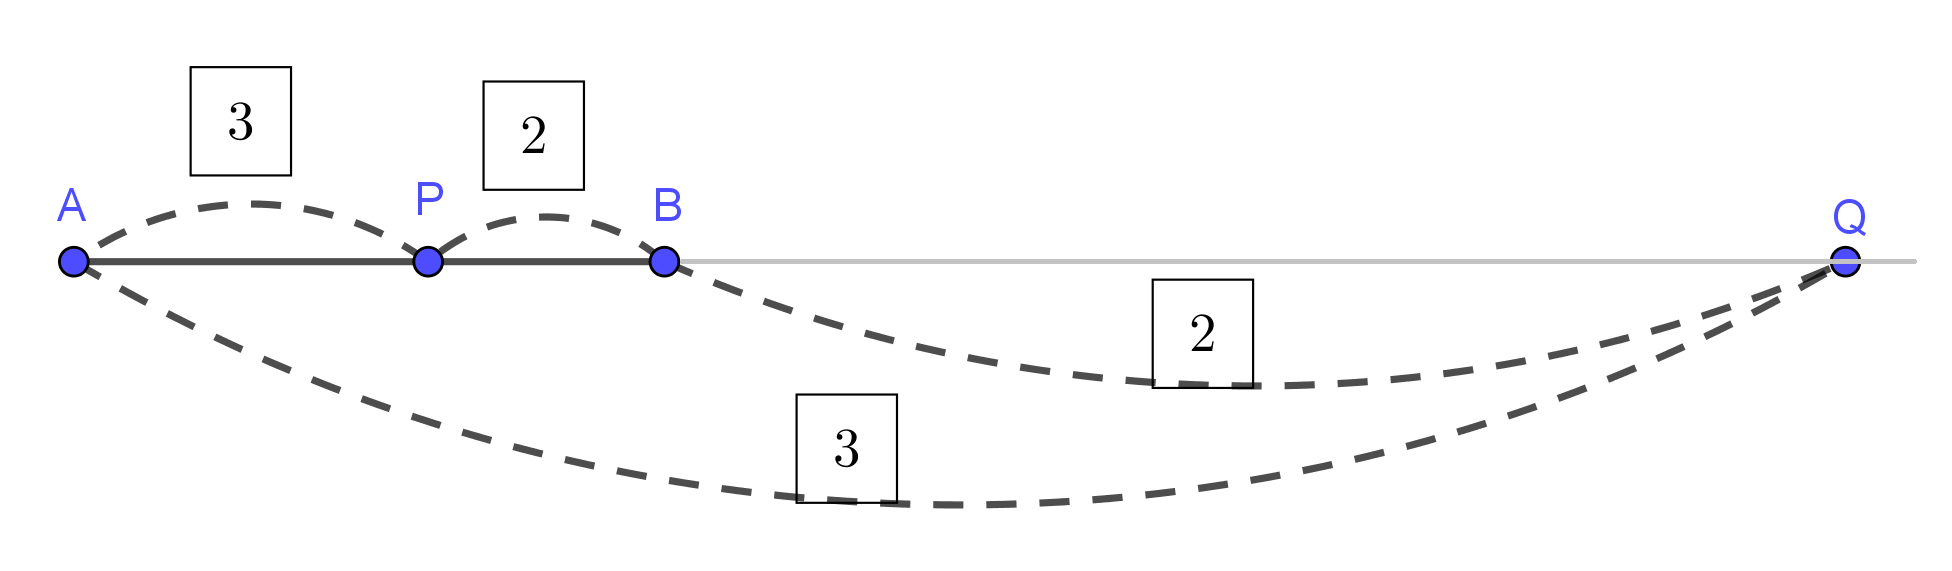
\includegraphics[width=0.6\textwidth]{int_15}
\end{center}
\procedure{0.1}

%%
\section{내분점과 외분점(2차원)}
%
\exam{}\label{intt01}
평면좌표 위의 두 점 \(A(-1,1)\), \(B(5,4)\)에 대해\\
(1) \(A\)와 \(B\)의 \(2:1\) 내분점은 \(P(3,3)\)이다.\par
\begin{center}
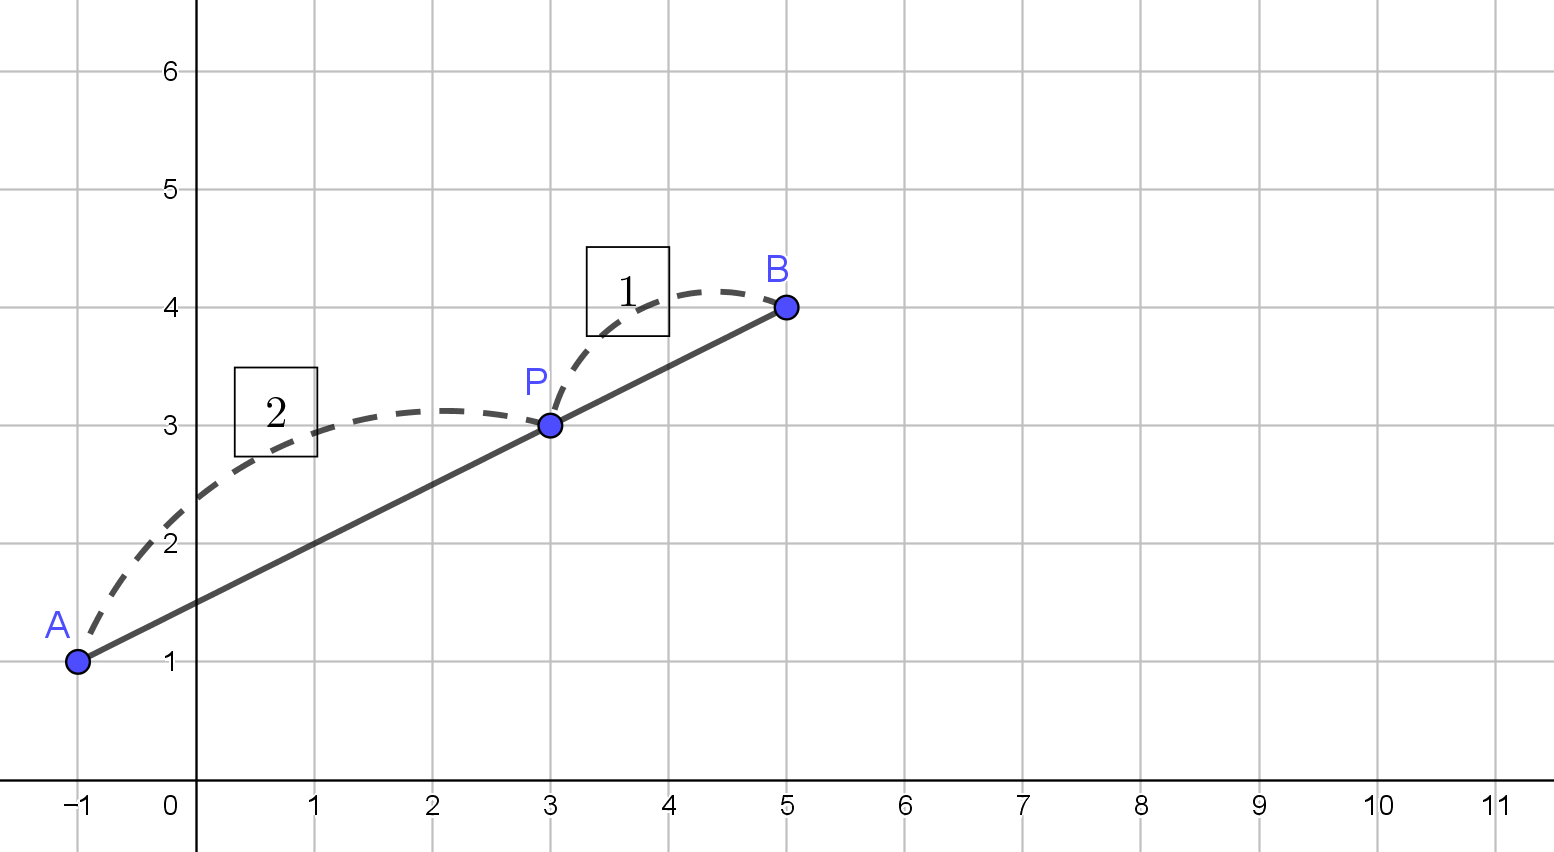
\includegraphics[width=0.65\textwidth]{intt_01}
\end{center}
(2) \(A\)와 \(B\)의 \(2:1\) 외분점은 \(Q(11,7)\)이다.
\begin{center}
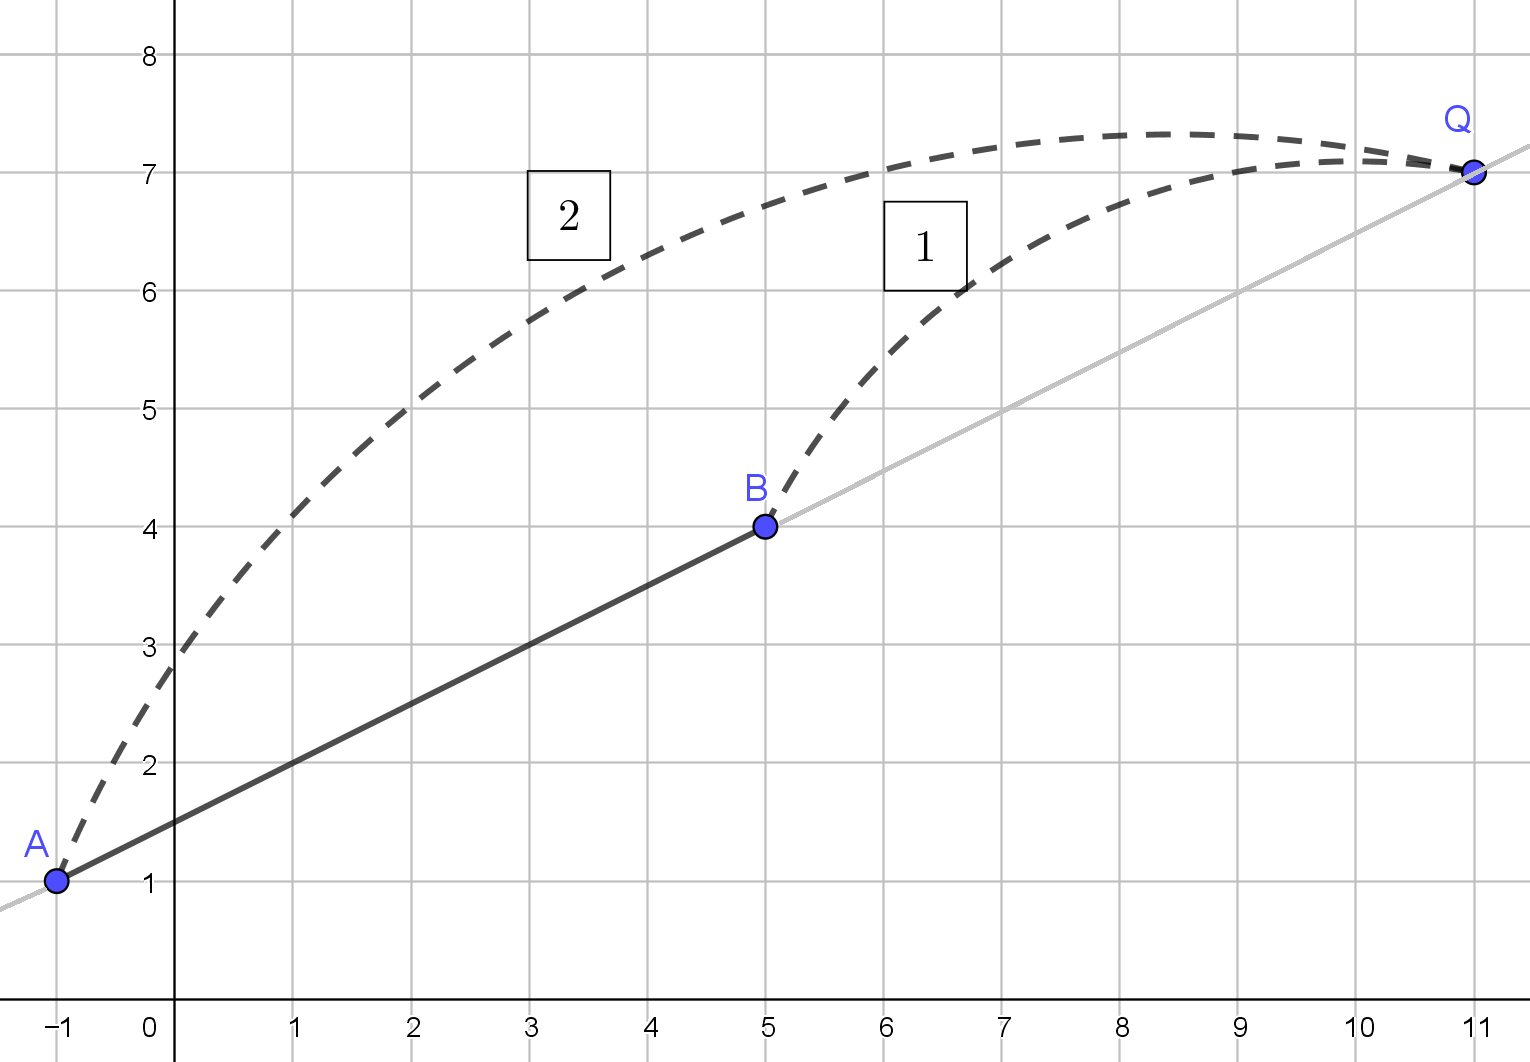
\includegraphics[width=0.65\textwidth]{intt_02}
\end{center}

%
\prob{}\label{intt03}
평면 좌표 위의 두 점 \(A(0,4)\) \(B(4,0)\)에 대해\\
(1) \(A\)와 \(B\)의 \(3:1\) 내분점 \(P\)\\
(2) \(A\)와 \(B\)의  \(3:1\) 외분점 \(Q\)\\
(3) \(A\)와 \(B\)의 \(1:2\) 외분점 \(R\)\\
의 좌표를 각각 구하여라.

%
\exam{}\label{intt04}
예시 \ref{intt01})에서 \(P=(x_1,y_1)\)로 놓고 다음과 같이 해석해보자.
\par\medskip\noindent
\(A\)에서 \(x\)축에 내린 수선의 발을 \(A'\)\\
\(B\)에서 \(x\)축에 내린 수선의 발을 \(B'\)\\
\(P\)에서 \(x\)축에 내린 수선의 발을 \(P'\)
\par\medskip\noindent
이라고 놓으면
\begin{center}
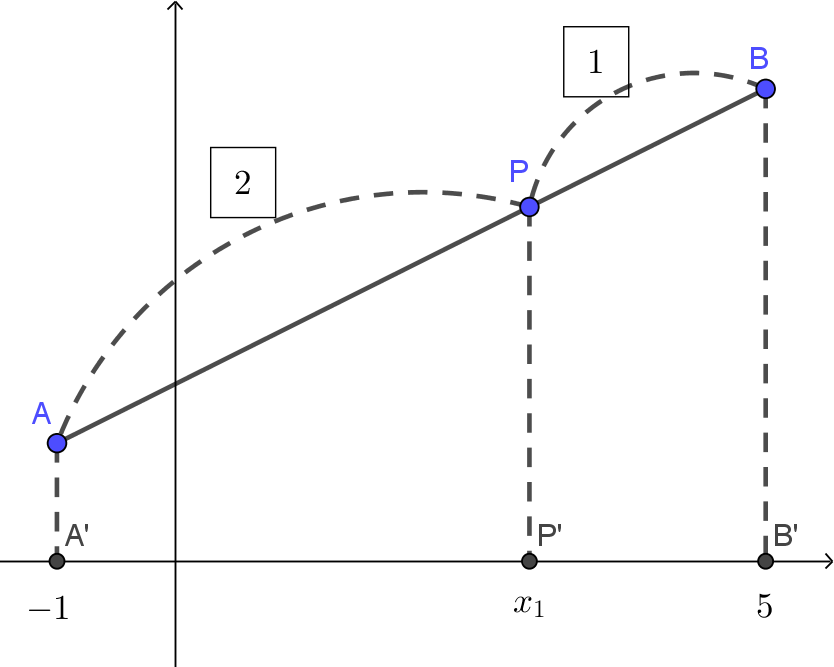
\includegraphics[width=0.4\textwidth]{intt_04}
\end{center}
닮음의 성질에 의해
\[\overline{A'P'}:\overline{P'B'}=2:1\]
이다.
즉 \(P'(x_1)\)은 \(A'(-1)\)와 \(B'(5)\)의 2:1 내분점이다.
따라서
\[x_1=\frac{2\times5+1\times(-1)}{2+1}=3\]

마찬가지로
\par\medskip\noindent
\(A\)에서 \(y\)축에 내린 수선의 발을 \(A''\)\\
\(B\)에서 \(y\)축에 내린 수선의 발을 \(B''\)\\
\(P\)에서 \(y\)축에 내린 수선의 발을 \(P''\)
\par\medskip\noindent
이라고 놓으면
\begin{center}
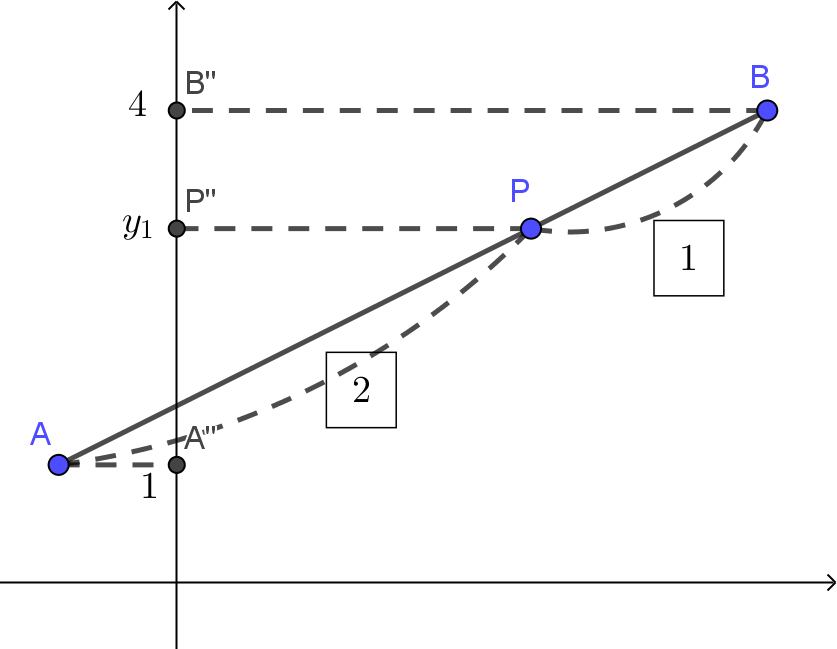
\includegraphics[width=0.4\textwidth]{intt_05}
\end{center}
\(P''(y_1)\)은 \(A''(1)\)와 \(B''(4)\)의 2:1 내분점이다.
\[y_1=\frac{2\times4+1\times1}{2+1}=3\]
즉
\[P=(x_1,y_1)=\left(\frac{2\times5+1\times(-1)}{2+1}\:\:,\frac{2\times4+1\times1}{2+1}\right)=(3,3)\]
이다.

같은 방법으로 외분점 \(Q\)는
\[Q=(q_1,q_2)=\left(\frac{2\times5-1\times(-1)}{2-1}\:\:,\frac{2\times4-1\times1}{2-1}\right)=(11,7)\]
로 계산할 수 있다.

\bigskip
%
\begin{mdframed}
\theo{내분점과 외분점의 좌표(2차원)}\label{intt06}
두 점 \(A(x_1,y_1)\), \(B(x_2,y_2)\)에 대하여
\(A\)와 \(B\)의 \(m:n\) 내분점 \(P\), 외분점 \(Q\)의 좌표는 각각
\[P=\left(\frac{mx_2+nx_1}{m+n}\:\:,\:\:\frac{my_2+ny_1}{m+n}\right)\]
\[Q=\left(\frac{mx_2-nx_1}{m-n}\:\:,\:\:\frac{my_2-ny_1}{m-n}\right)\]
이다.
\end{mdframed}

%
\prob{}\label{intt07}
문제 \ref{intt03})를 정리 \ref{intt06})의 공식을 사용하여 풀어라.

%
\prob{}\label{intt08}
평면 위의 점 \(P\)가 \(A(3,-3)\)와 \(B(8,7)\)의 \(3:2\) 내분점일 때, \(P\)의 좌표를 구하여라.
\procedure{0.1}

%
\prob{}\label{intt09}
평면 위의 점 \(P\)가 \(A(1,0)\)와 \(B(3,-1)\)의 \(2:1\) 외분점일 때, \(P\)의 좌표를 구하여라.
\procedure{0.1}

%
\prob{}\label{intt10}
평면 위의 점 \(P(3,-2)\)가 \(A(0,7)\)와 \(B\)의 \(3:1\) 내분점일 때, \(B\)의 좌표를 구하여라.
\procedure{0.1}

%
\prob{}\label{intt11}
평면 위의 세 점 \(A(5,7)\), \(B(-1,2)\), \(C(8,5)\)로 만든 삼각형 \(\triangle ABC\)이 있다.
선분 \(\ov BC\) 위에 \(B\)와 \(C\)의 \(2:1\) 내분점 \(D\)를 잡고
선분 \(\ov AD\) 위에 \(A\)와 \(D\)의 \(1:2\) 내분점 \(E\)를 잡을 때
\(E\)의 좌표를 구하여라.
\procedure{0.1}

%%
\section{중점과 무게중심}

두 점 \(A\), \(B\)의 \emph{중점}이란, 두 점의 1:1 내분점을 말한다.

\bigskip
정리 \ref{int07})와 정리 \ref{intt06})에 \(m=1\), \(n=1\)을 대입하면 다음 결과를 얻는다.
%
\begin{mdframed}
\theo{두 점 \(A\), \(B\)의 중점}\label{mid01}
\begin{enumerate}
\item
수직선 위의 두 점 \(A(a)\), \(B(b)\)의 중점 \(M\)의 좌표는
\[M=\left(\frac{a+b}2\right)\]
이다.
\item
평면 위의 두 점 \(A(x_1,y_1)\), \(B(x_2,y_2)\)의 중점 \(M\)의 좌표는
\[M=\left(\frac{x_1+x_2}2\:\:,\:\:\frac{y_1+y_2}2\right)\]
이다.
\end{enumerate}
\end{mdframed}

%
\prob{}\label{mid02}
수직선 위의 두 점 \(A(4)\), \(B(b)\)의 중점이 \(M(10)\)일 때, \(b\)의 값을 구하여라.
\procedure{0.1}

%
\prob{}\label{mid03}
평면 위의 두 점 \(A(1,10)\), \(B(5,6)\)의 중점 \(M\)의 좌표를 구하여라.
\procedure{0.1}

%%
%\prob{}\label{mid04}
%수직선 위의 두 점 \(O(0)\), \(A(1)\)에 대하여\\
%점\(O\)와 점 \(A\)의 중점을 \(A_1\)\\
%점\(O\)와 점 \(A_1\)의 중점을 \(A_2\)\\
%점\(O\)와 점 \(A_2\)의 중점을 \(A_3\)\\
%점\(O\)와 점 \(A_3\)의 중점을 \(A_4\)\\
%\(\vdots\)\\
%으로 정할 때, \(A_{10}\)의 좌표를 \(a\)라 할 때, \(a\)의 값을 구하여라. 
%\procedure{0.1}

삼각형 \(ABC\)의 무게중심 \(G\)는 세 중선의 교점이다.
또한, 한 중선을 \(2:1\)로 내분한 점이기도 하다.
따라서 다음을 얻는다.
%
\begin{mdframed}
\theo{삼각형 \(ABC\)의 무게중심}\label{mid04}
평면 위의 세 점 \(A(x_1,y_1)\), \(B(x_2,y_2)\), \(C(x_3,y_3)\)의 무게중심 \(G\)의 좌표는
\[G=\left(\frac{x_1+x_2+x_3}3\:\:,\:\:\frac{y_1+y_2+y_3}3\right)\]
이다.
\end{mdframed}

\begin{center}
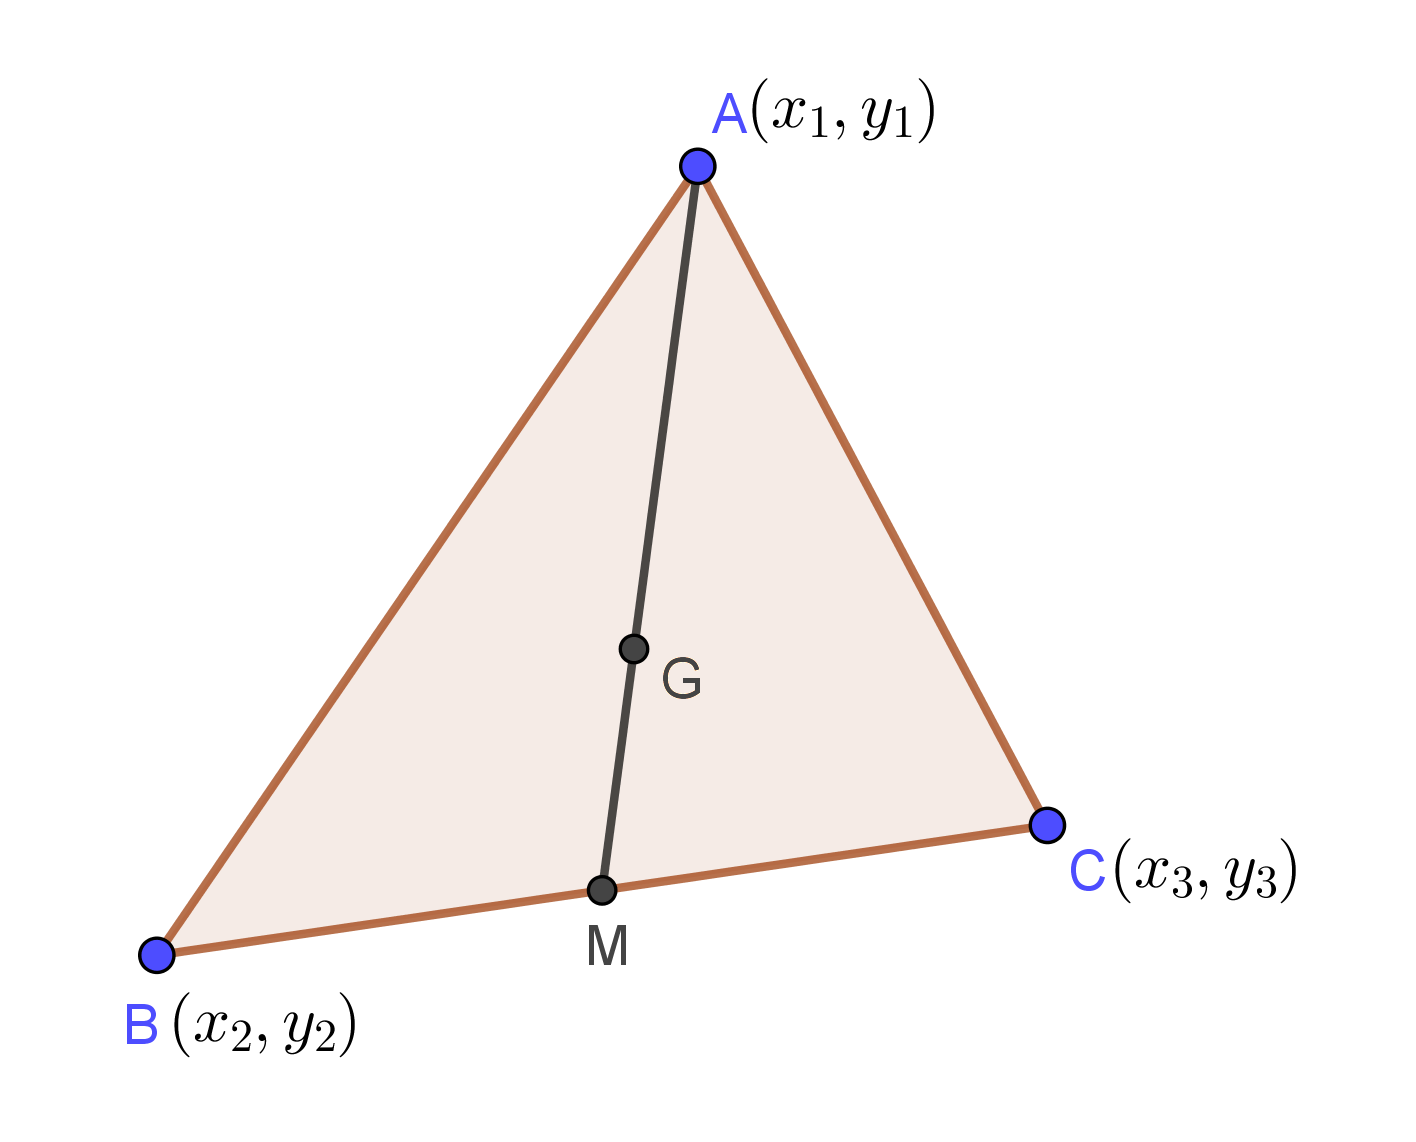
\includegraphics[width=0.4\textwidth]{mid_04}
\end{center}

%
\proo
\(B\)와 \(C\)의 중점을 \(M\)이라 하면
\[M=\left(\frac{x_1+x_2}2,\frac{y_1+y_2}2\right)\]
이다.
무게중심 \(G\)는 \(A\)와 \(M\)의 2:1 내분점이므로
\begin{align*}
G
&=\left(\frac{2\cdot\frac{x_1+x_2}2+1\cdot x_3}{2+1},
\frac{2\cdot\frac{y_1+y_2}2+1\cdot y_3}{2+1}\right)\\
&=\left(\frac{x_1+x_2+x_3}3\:\:,\:\:\frac{y_1+y_2+y_3}3\right)
\end{align*}
\qed

\clearpage
%
\prob{}\label{mid05}
평면 위의 세 점 \(A(1,5)\), \(B(-2,1)\), \(C(7,3)\)의 무게중심 \(G\)의 좌표를 구하여라.
\procedure{0.1}

%
\prob{}\label{mid06}
평면 위의 세 점 \(A(a,3)\), \(B(3,b)\), \(C(12,0)\)의 무게중심 \(G\)의 좌표가 \(G=(8,0)\)일 때, \(a+b\)의 값을 구하여라.하여라.
\procedure{0.1}

%%
\section*{답}
\addcontentsline{toc}{chapter}{\protect\numberline{*}답}

\begin{minipage}[t]{.49\textwidth}
%
\an{int03}
\begin{enumerate}
\item
\(P(8)\)
\item
\(Q(14)\)
\item
\(R(-6)\)
\end{enumerate}
참고 :\\
\begin{center}
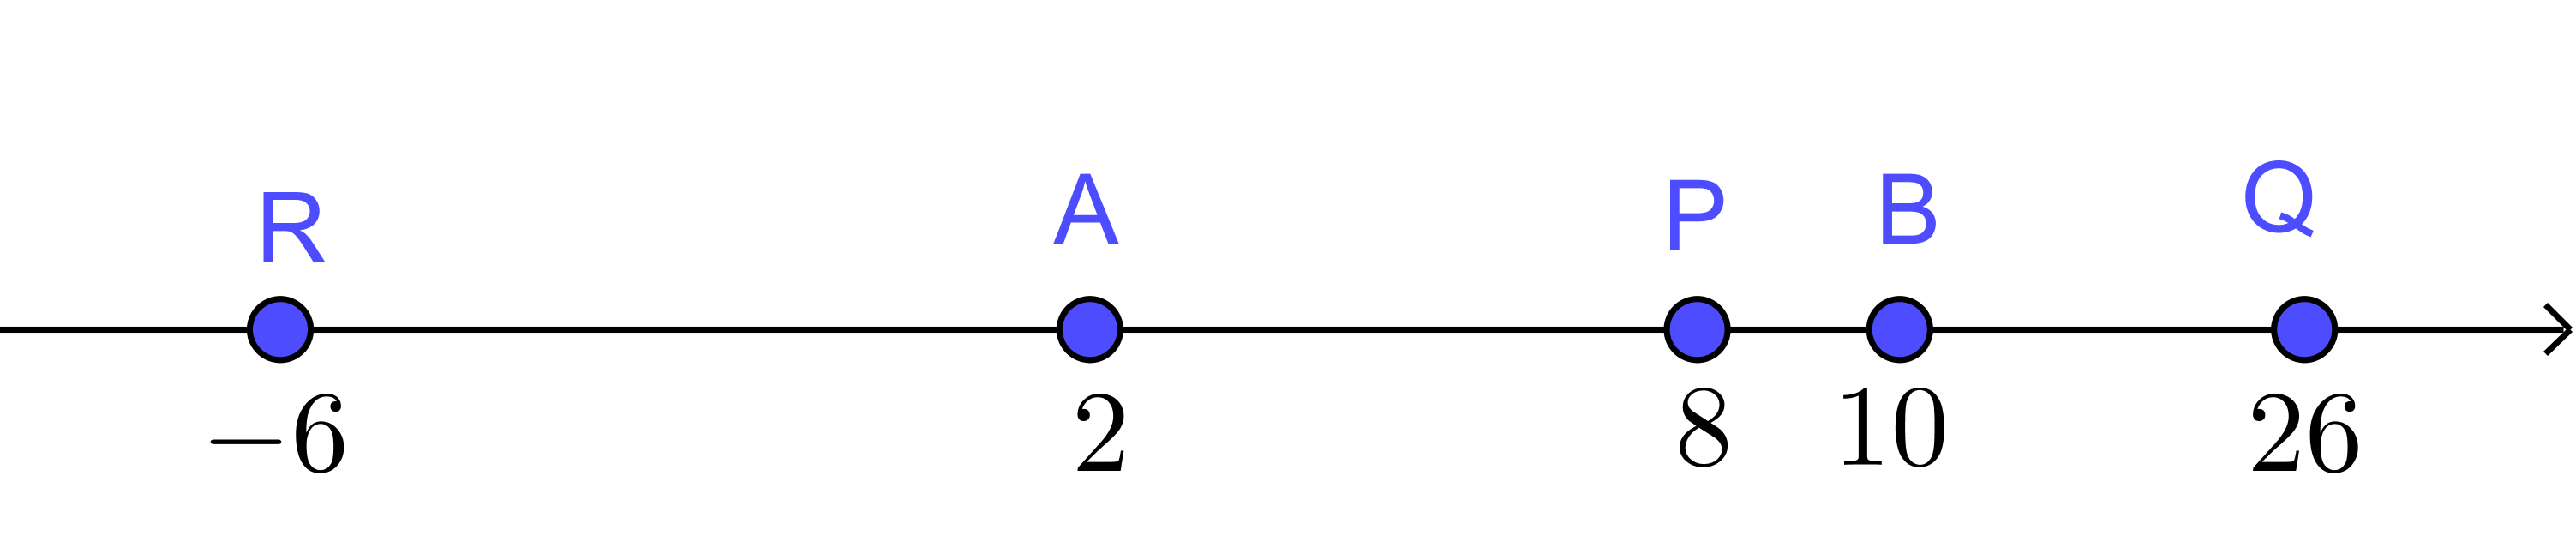
\includegraphics[width=0.9\textwidth]{int_03}
\end{center}


%
\an{int06}
생략

%
\an{int10}
생략

%
\an{int11}
\begin{enumerate}
\item
\(2:3\)
\item
\(2:1\)
\item
\(3:1\)
\end{enumerate}

%
\an{int12}
\(18\)
%\begin{gather*}
%9=\frac{2\times b+3\times3}{2+3}\\
%45=2b+9\\
%b=18
%\end{gather*}

%
\an{int13}
\(3\)
%\begin{gather*}
%11=\frac{4\times5-3\times3a}{4-3}\\
%11=20-9a\\
%a=3
%\end{gather*}

\end{minipage}
\begin{minipage}[t]{0.49\textwidth}
%
\an{int14}
\(3:1:2\)
%선분 \(\ov AB\)의 길이를 \(a\)라고 하면\\
%\(\ov AP=\frac12a\), \(\ov QB=\frac13a\),\\
%\(\ov PQ=1-\ov AP-\ov QB=\frac16a\)\\
%따라서
%\begin{align*}
%\ov AP:\ov PQ:\ov QB
%&=\frac12a:\frac16a:\frac13a\\
%&=3:1:2
%\end{align*}

%
\an{int15}
\(3:2:10\)
%선분 \(\ov AB\)의 길이를 \(a\)라고 하면\\
%\(\ov AP=\frac35a\), \(\ov PB=\frac25a\), \(\ov BQ=2a\)\\
%따라서 
%\begin{align*}
%\ov AP:\ov PB:\ov BQ
%&=\frac35a:\frac25a:2a\\
%&=3:2:10
%\end{align*}

%
\an{intt03}
\begin{enumerate}
\item
\(P=(3,1)\)
\item
\(Q=(6,-2)\)
\item
\(R=(-4,8)\)
\end{enumerate}
참고 :\\
\begin{center}
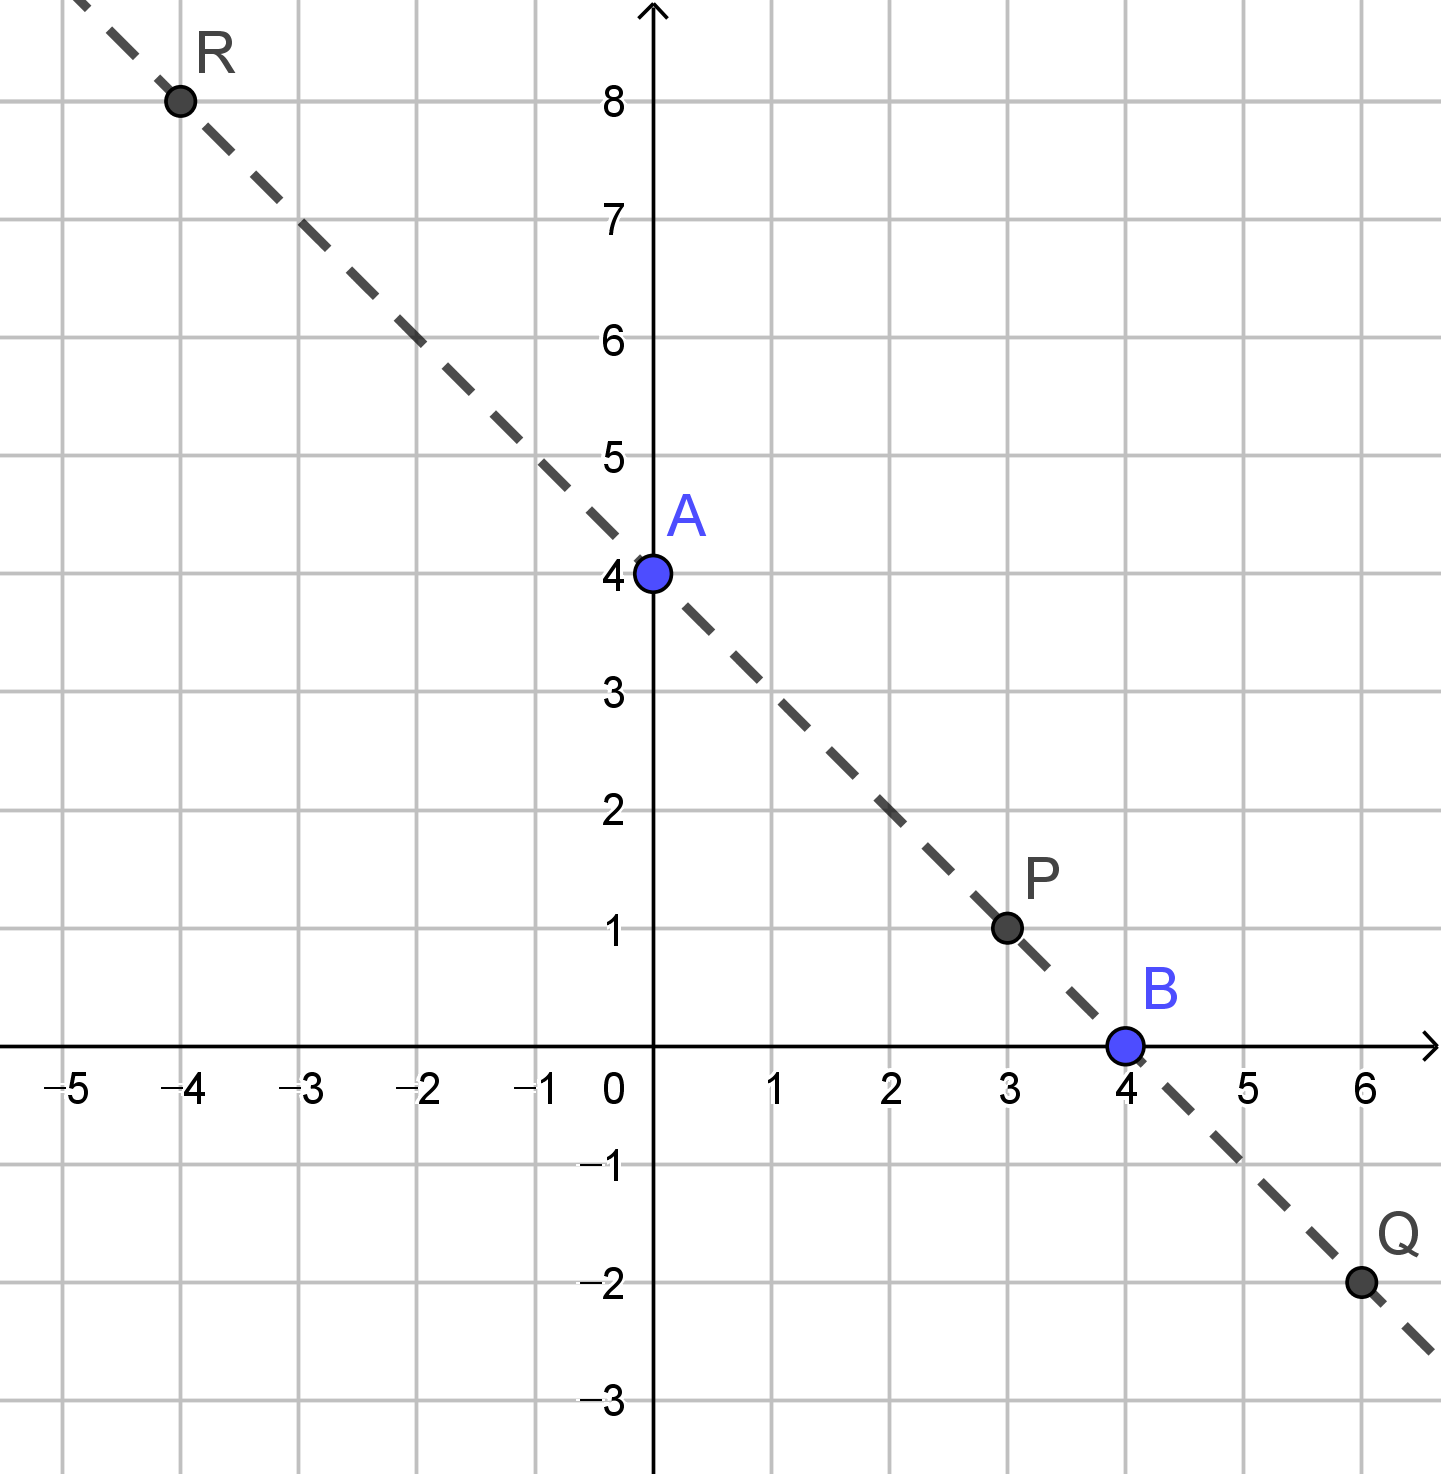
\includegraphics[width=0.9\textwidth]{intt_03}
\end{center}

%
\an{intt07}
생략

%
\an{intt08}
\(P=(6,3)\)

\end{minipage}
\clearpage
\begin{minipage}[t]{0.49\textwidth}

%
\an{intt09}
\(P=(5,-2)\)

%
\an{intt10}
\(B=(4,-5)\)

%
\an{intt11}
\(E=(5,6)\)

%
\an{mid02}
\(b=16\)

%
\an{mid03}
\(M=(3,8)\)

%%
%\an{mid04}
%\(a=\frac1{1024}\) 혹은 \(a=\left(\frac12\right)^{10}\)

%
\an{mid05}
\(G=(2,3)\)

%
\an{mid06}
\(6\)
\end{minipage}

\end{document}